\begin{frame}[label=title]
    \centering
    \begin{figure}[H]
        
\includegraphics[keepaspectratio, width=0.7\paperwidth, height=\paperheight]{Logos/LeeLogo}
    \end{figure}
    Informatik: Data Science und Sicherheit\\
    \emoji{clamp}\textbf{Kompression}: Huffman-Kompression
\end{frame}

\begin{frame}{Huffman-Kodierung}
	\textbf{Idee}: Immer zuerst Knoten mit kleinsten Prozentzahlen verbinden\\[.5cm]
\end{frame}

\begin{frame}{Huffman-Kodierung: Algorithmus}
	\begin{itemize}[<+->]
		\small
		\item Jeder Buchstabe wird als Graph mit einem Knoten (=Baum mit einem Blatt) betrachtet. Die Häufigkeit jedes Buchstabens wird neben dem Blatt notiert. Wir wollen nun die Buchstaben zu Teilbäumen verbinden, bis wir einen einzigen Baum haben.
		\begin{figure}[H]
			\footnotesize
			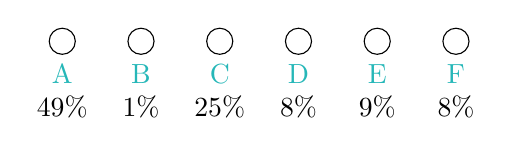
\begin{tikzpicture}
				\tikzstyle{n} = [text width=1cm,align=center, draw, shape=circle]
				\node[circle,draw, label={[align=center]below:\textcolor{BlueGreen}{A}\\ 49\%}, ](a){};
				\node[circle,draw, label={[align=center]below:\textcolor{BlueGreen}{B}\\ 1\%}, right of=a](b){};
				\node[circle,draw, label={[align=center]below:\textcolor{BlueGreen}{C}\\ 25\%}, right of=b](c){};
				\node[circle,draw, label={[align=center]below:\textcolor{BlueGreen}{D}\\ 8\%}, right of=c](d){};
				\node[circle,draw, label={[align=center]below:\textcolor{BlueGreen}{E}\\ 9\%}, right of=d](e){};
				\node[circle,draw, label={[align=center]below:\textcolor{BlueGreen}{F}\\ 8\%}, right of=e](f){};
			\end{tikzpicture}
			\normalsize
		\end{figure}
		\item In einer Schleife: Wir schauen alle isolierten Blätter und Wurzeln von Teilbäumen an. Diejenigen  Knoten, die die kleinste (gemeinsame) Prozentzahl enthalten werden miteinander verbunden. Die neue Wurzel wird markiert mit dem Prozentsatz beider Knoten.
		\begin{figure}[H]
			\footnotesize
			\begin{tikzpicture}[-,>=stealth',
				level distance=12mm,
				level 1/.style={sibling distance=15mm},
				level 2/.style={sibling distance=30mm},
				level 3/.style={sibling distance=15mm},
				level 4/.style={sibling distance=15mm},
				level 5/.style={sibling distance=15mm},
				leaf/.style={circle, draw},
				edge from parent path={(\tikzparentnode.south) -- (\tikzchildnode)}] 
				
				
				\usetikzlibrary{shapes}
				\tikzstyle{n} = [text width=1cm,align=center]
				\tikzstyle{r} = [text=red]
				
				\node[n]{\textcolor{BlueGreen}{B,D}\\ 9\%}[edge from parent]
				child {node[n] {\textcolor{BlueGreen}{B}\\ 1\%}
					edge from parent node[left,r]{};
				}
				child {node[n]{\textcolor{BlueGreen}{D}\\ 8\%}
					edge from parent node[r,right]{};
				};
			\end{tikzpicture}
			\normalsize
		\end{figure}
		\item Falls mehrere Möglichkeiten mit gleicher relativer Häufigkeit existieren, nehmen wir den Teilbaum mit der geringsten Tiefe.
		\end{itemize}
		\only<4>{\textbf{Welche Knoten werden als nächstes miteinander verbunden?}}
\end{frame}

\begin{frame}{Huffman-Kodierung: Beispiel}
	\begin{figure}[H]
		\footnotesize
		\begin{tikzpicture}[-,>=stealth',
			level distance=15mm,
			level 1/.style={sibling distance=15mm},
			level 2/.style={sibling distance=30mm},
			level 3/.style={sibling distance=15mm},
			level 4/.style={sibling distance=15mm},
			level 5/.style={sibling distance=15mm},
			leaf/.style={circle, draw},
			edge from parent path={(\tikzparentnode.south) -- (\tikzchildnode)}] 
			
			
			\usetikzlibrary{shapes}
			\tikzstyle{n} = [text width=1cm,align=center]
			\tikzstyle{r} = [text=red]

			\node(bd)[n]{\textcolor{BlueGreen}{B,D}\\ 9\%}[edge from parent]
			child {node(b)[n] {\textcolor{BlueGreen}{B}\\ 1\%}
				edge from parent node[left,r]{} ;
			}
			child {node[n]{\textcolor{BlueGreen}{D}\\ 8\%}
				edge from parent node[r,right]{};
			};
			\node(ef)[n, left of=bd,xshift=-15mm]{\textcolor{BlueGreen}{E,F}\\ 17\%}[edge from parent]
			child {node(f)[n] {\textcolor{BlueGreen}{F}\\ 8\%}
				edge from parent node[left,r]{} ;
			}
			child {node[n]{\textcolor{BlueGreen}{E}\\ 9\%}
				edge from parent node[r,right]{};
			};
			\node[n, left of=f](c){\textcolor{BlueGreen}{C}\\ 25\%};
			\node[n, left of=c](a){\textcolor{BlueGreen}{A}\\ 49\%};
		\end{tikzpicture}
		\normalsize
	\end{figure}
	\centering
	$\rightarrow$ Weshalb haben wir einen Baum \{\textcolor{BlueGreen}{E,F}\} statt \{\textcolor{BlueGreen}{F,B,D}\} gemacht?
\end{frame}


\begin{frame}{Huffman-Kodierung: Beispiel}
	\begin{figure}[H]
		\footnotesize
		\begin{tikzpicture}[-,>=stealth',
			level distance=15mm,
			level 1/.style={sibling distance=30mm},
			level 2/.style={sibling distance=15mm},
			level 3/.style={sibling distance=15mm},
			level 4/.style={sibling distance=15mm},
			level 5/.style={sibling distance=15mm},
			leaf/.style={circle, draw},
			edge from parent path={(\tikzparentnode.south) -- (\tikzchildnode)}] 
			
			\usetikzlibrary{shapes}
			\tikzstyle{n} = [text width=1cm,align=center]
			\tikzstyle{r} = [text=red]
			
			\node(febd)[n]{\textcolor{BlueGreen}{F,E,B,D}\\ 26\%}[edge from parent]
				child{node(ef)[n]{\textcolor{BlueGreen}{E,F}\\ 17\%}
					child {node(f)[n] {\textcolor{BlueGreen}{F}\\ 8\%}
						edge from parent node[left,r]{} ;
					}
					child {node[n]{\textcolor{BlueGreen}{E}\\ 9\%}
						edge from parent node[r,right]{};
					}
					edge from parent node[r,right]{};
				}
				child{node(bd)[n]{\textcolor{BlueGreen}{B,D}\\ 9\%}
					child {node(b)[n] {\textcolor{BlueGreen}{B}\\ 1\%}
						edge from parent node[left,r]{} ;
					}
					child {node[n]{\textcolor{BlueGreen}{D}\\ 8\%}
						edge from parent node[r,right]{};
					}
					edge from parent node[r,left]{};
				};
			\node[n, left of=f](c){\textcolor{BlueGreen}{C}\\ 25\%};
			\node[n, left of=c](a){\textcolor{BlueGreen}{A}\\ 49\%};
		\end{tikzpicture}
		\normalsize
	\end{figure}
\end{frame}

\begin{frame}{Huffman-Kodierung: Beispiel}
	\begin{figure}[H]
		\footnotesize
		\begin{tikzpicture}[-,>=stealth',
			level distance=15mm,
			level 1/.style={sibling distance=60mm},
			level 2/.style={sibling distance=30mm},
			level 3/.style={sibling distance=30mm},
			level 4/.style={sibling distance=15mm},
			level 5/.style={sibling distance=15mm},
			leaf/.style={circle, draw},
			edge from parent path={(\tikzparentnode.south) -- (\tikzchildnode)}] 
			
			\usetikzlibrary{shapes}
			\tikzstyle{n} = [text width=1cm,align=center]
			\tikzstyle{r} = [text=red]
			
			\node(acebd)[n]{\textcolor{BlueGreen}{A,C,F,E,B,D}\\ 100\%}[edge from parent]
			child{node(a)[n]{\textcolor{BlueGreen}{A}\\ 49\%}
				edge from parent node[left,r]{} ;
			}
			child{node(cfebd)[n]{\textcolor{BlueGreen}{C,F,E,B,D}\\ 51\%}
				child{node(c)[n]{\textcolor{BlueGreen}{C}\\ 25\%}
					edge from parent node[left,r]{} ;
					}
				child{node(febd)[n]{\textcolor{BlueGreen}{F,E,B,D}\\ 26\%}
					child{node(ef)[n]{\textcolor{BlueGreen}{E,F}\\ 17\%}
						child {node(f)[n] {\textcolor{BlueGreen}{F}\\ 8\%}
							edge from parent node[left,r]{} ;
						}
						child {node[n]{\textcolor{BlueGreen}{E}\\ 9\%}
							edge from parent node[r,right]{};
						}
						edge from parent node[r,right]{};
					}
					child{node(bd)[n]{\textcolor{BlueGreen}{B,D}\\ 9\%}
						child {node(b)[n] {\textcolor{BlueGreen}{B}\\ 1\%}
							edge from parent node[left,r]{} ;
						}
						child {node[n]{\textcolor{BlueGreen}{D}\\ 8\%}
							edge from parent node[r,right]{};
						}
						edge from parent node[r,left]{};
					}
				edge from parent node[right,r]{};
				}
				edge from parent node[right,r]{};
			};		
		\end{tikzpicture}
		\normalsize
	\end{figure}
	\centering
	$\rightarrow$ Welcher Binärcode hat \textcolor{BlueGreen}{B}? Welcher hat \textcolor{BlueGreen}{E}?
\end{frame}

\begin{frame}{Huffman-Kodierung: Beispiel}
	\begin{figure}[H]
		\footnotesize
		\begin{tikzpicture}[-,>=stealth',
			level distance=15mm,
			level 1/.style={sibling distance=60mm},
			level 2/.style={sibling distance=30mm},
			level 3/.style={sibling distance=30mm},
			level 4/.style={sibling distance=15mm},
			level 5/.style={sibling distance=15mm},
			leaf/.style={circle, draw},
			edge from parent path={(\tikzparentnode.south) -- (\tikzchildnode)}] 
			
			\usetikzlibrary{shapes}
			\tikzstyle{n} = [text width=1cm,align=center]
			\tikzstyle{r} = [text=red]
			
			\node(acebd)[n]{\textcolor{BlueGreen}{A,C,F,E,B,D}\\ 100\%}[edge from parent]
			child{node(a)[n]{\textcolor{BlueGreen}{A}\\ 49\%\\\textcolor{red}{0}}
				edge from parent node[left,r]{0} ;
			}
			child{node(cfebd)[n]{\textcolor{BlueGreen}{C,F,E,B,D}\\ 51\%}
				child{node(c)[n]{\textcolor{BlueGreen}{C}\\ 25\%\\\textcolor{red}{10}}
					edge from parent node[left,r]{0} ;
				}
				child{node(febd)[n]{\textcolor{BlueGreen}{F,E,B,D}\\ 26\%}
					child{node(ef)[n]{\textcolor{BlueGreen}{E,F}\\ 17\%}
						child {node(f)[n] {\textcolor{BlueGreen}{F}\\ 8\%\\\textcolor{red}{1100}}
							edge from parent node[left,r]{0} ;
						}
						child {node[n]{\textcolor{BlueGreen}{E}\\ 9\%\\\textcolor{red}{1101}}
							edge from parent node[r,right]{1};
						}
						edge from parent node[r,left]{0};
					}
					child{node(bd)[n]{\textcolor{BlueGreen}{B,D}\\ 9\%}
						child {node(b)[n] {\textcolor{BlueGreen}{B}\\ 1\%\\\textcolor{red}{1110}}
							edge from parent node[left,r]{0} ;
						}
						child {node[n]{\textcolor{BlueGreen}{D}\\ 8\%\\\textcolor{red}{1111}}
							edge from parent node[r,right]{1};
						}
						edge from parent node[r,right]{1};
					}
					edge from parent node[right,r]{1};
				}
				edge from parent node[right,r]{1};
			};		
		\end{tikzpicture}
		\normalsize
	\end{figure}
	\centering
\end{frame}

\begin{frame}{Fazit}
	\begin{itemize}
		\item Strategie der \textbf{Maximale Balance}: \textit{top-down}-Ansatz (von Wurzel zu Blättern), kann zu suboptimalen Kodierungen führen
		\item \textbf{Huffman-Kodierung}: \textit{bottom-up}-Ansatz (von Blättern zur Wurzel), garantiert bestmögliche Kodierungslänge für alle Buchstaben
	\end{itemize}
\end{frame}

\begin{frame}[label=auftrag]{Auftrag}
	\begin{itemize}
		\item \aufgabebox{Aufgaben 1.6 - 1.9}
	\end{itemize}
\end{frame}
